\documentclass{article}
\usepackage{graphicx} % Required for inserting images
\usepackage[margin=0.75in]{geometry}
\usepackage{xcolor}
\title{140.644 Note -- In Class}
\author{Moran Guo}
\date{August 2024}

\begin{document}

\maketitle

\section{Aug 29th}

Consider a linear model: $$\hat{f}(X) = \hat{\beta}_0 + \hat{\beta}_1 X + \hat{\beta}_2 X + \hat{\beta}_3 X + \hat{\beta}_4 X + \hat{\beta}_5 X$$

How do we simplify it?\\

1. Sparsity of the parameters: Removing one (or more) variables.\\

2. Use non-linear models to re-model the outcome variable.\\

\noindent Flexibility vs. Interpret-ability\\

Increasing the flexibility \textbf{generalize the model}, but makes the model \textbf{harder to interpret}. -- How do we keep a balance between these two?\\

It seems that methods such as Trees and Generalized Additive Models keep a good balance between these two.\\

\noindent \textbf{Assessing Model Accuracy}\\

We could compute the Avg. MSE over training set ($\mathrm{Tr}$): $$\mathrm{MSE_{Tr}} = \mathrm{Ave_{i \in Tr}}[y_i - \hat{f}(x_i)]^2,$$

but this may be biased toward more over-fit models. Instead, we should use a new test data $\mathrm{Te} = \{x_i, y_i\}_1^M$ and calculate $$\mathrm{MSE_{Te}} = \mathrm{Ave_{i \in Te}}[y_i - \hat{f}(x_i)]^2.$$

In reality, the scenario is much more complex about how to decide the training and testing sets.

(If it's binary or classification problems, we could look at False Negative rate, False Positive rate, or misclassification \%).
\newpage
\begin{figure}[h!]
    \centering
    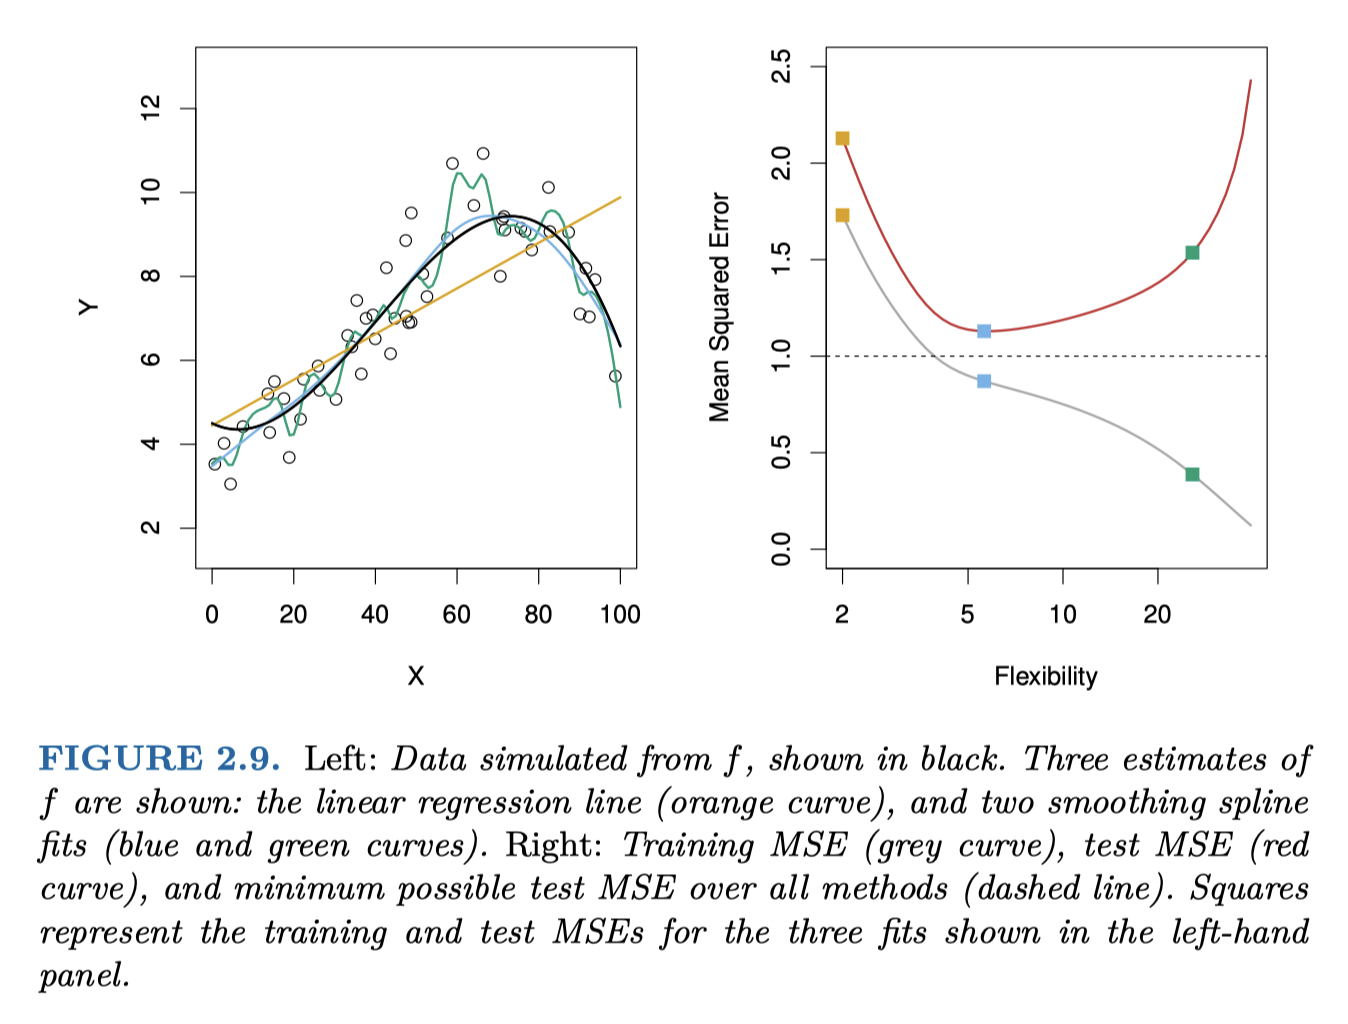
\includegraphics[width=0.75\linewidth]{Training_vs._Testing.png}
    \label{fig:train-vs-test}
\end{figure}

The \textcolor{blue}{blue} smoothing spline fit seems to perform the best across all three models. The \textcolor{green}{green} curve seems to have too much degrees of freedom by increasing the complexity of the model, which over-fits. In reality we are often time observing this U-shaped curve, where the overall MSE decreases when the complexity increase, but when the model is too complex, the $\mathrm{MSE_{Tr}}$ increases.\\

\noindent \textbf{Bias-Variance Trade-off}

Suppose we fit a model $\hat{f}(x)$ to training data $\mathrm{Tr}$, and let $(x_0, y_0)$ be an observation from the population. Then we have $$E\Big(y_0 - \hat{f}(x_0)\Big)^2 = \mathrm{Var}(\hat{f}(x_0)) + \Big[\mathrm{Bias}(\hat{f}(x_0))\Big]^2 + \mathrm{Var}(\epsilon).$$

\begin{figure}[h!]
    \centering
    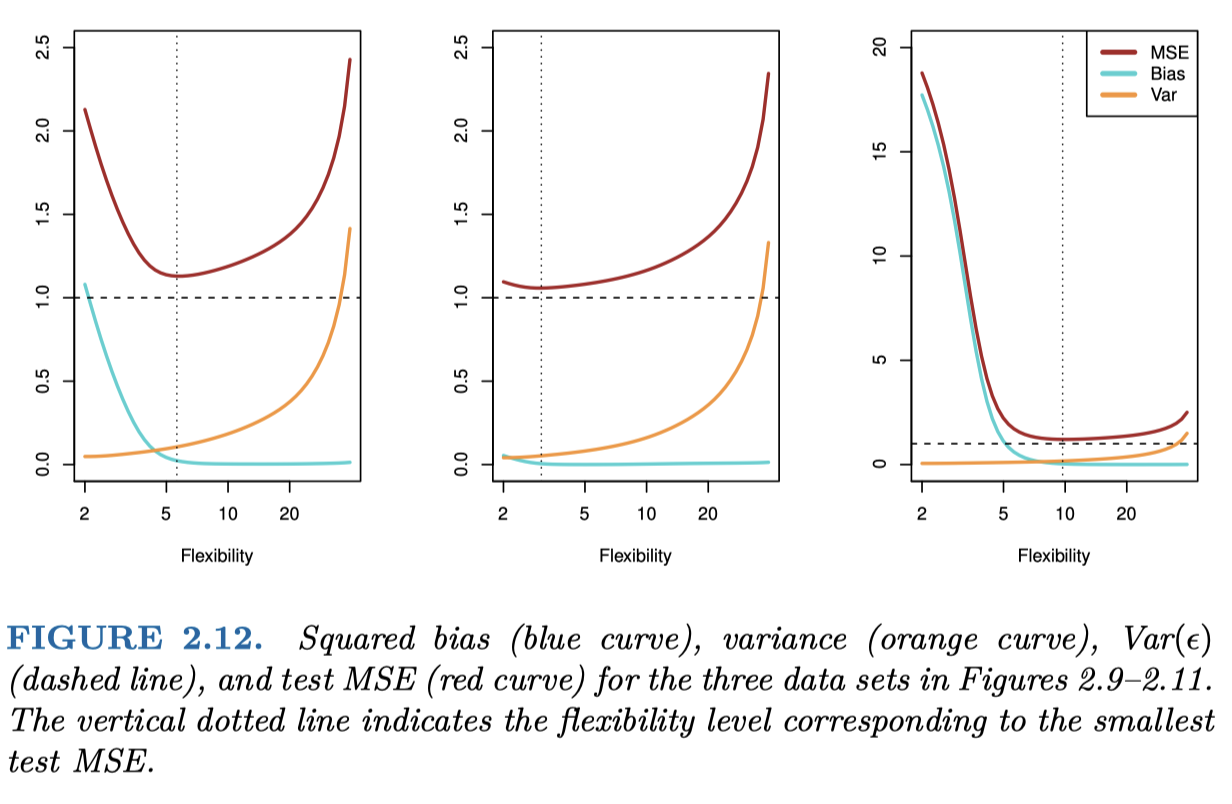
\includegraphics[width=0.75\linewidth]{bias_variance_tradeoff.png}
    \label{Bias-variance-tradeoff}
\end{figure}

As we are using more flexible model, the variance will increase and bias will decrease. But we generally have local minima to find the $\mathrm{MSE_{\min}}$.\\

\noindent \textbf{Classification Problem}

Response variable $Y$ is qualitative. Goal:
\begin{enumerate}
    \item Build a classifier $C(X)$ that assigns a class label from $\mathcal{C}$ to an unlabeled observation $X$.
    \item Assessing the uncertainty in each classification.
    \item Understand the roles of different predictors among $X$.
\end{enumerate}

To find the ideal $C(X)$, for $K$ elements in $\mathcal{C}$ numbered $1, 2, \cdots, K$. Let $$p_k(X) = \mathrm{Pr}(Y=k \vert X = x), k \in [1,K].$$

These are the conditional class probabilities at $x$; Then the \textbf{Bayes optimal classifier} at $x$ is $$C(x) = j$$  if $$p_j(x) = \max\{p_k(x)\}, k \in [1,K].$$\\

Nearest-neighbor averaging can also be used, especially when data is sparse.\\

\noindent \textbf{How good the model is} (classification model)?

Misclassification error rate: $$\mathrm{Err_{Te}} = \mathrm{Ave_{i \in Te}}I[y_i \neq \hat{C}(x_i)]$$

Pay attention to \textbf{selection bias} when having an \textbf{extremely low} misclassification rate.\\

\noindent \textbf{K-nearest Neighbors}
\begin{figure}[h!]
    \centering
    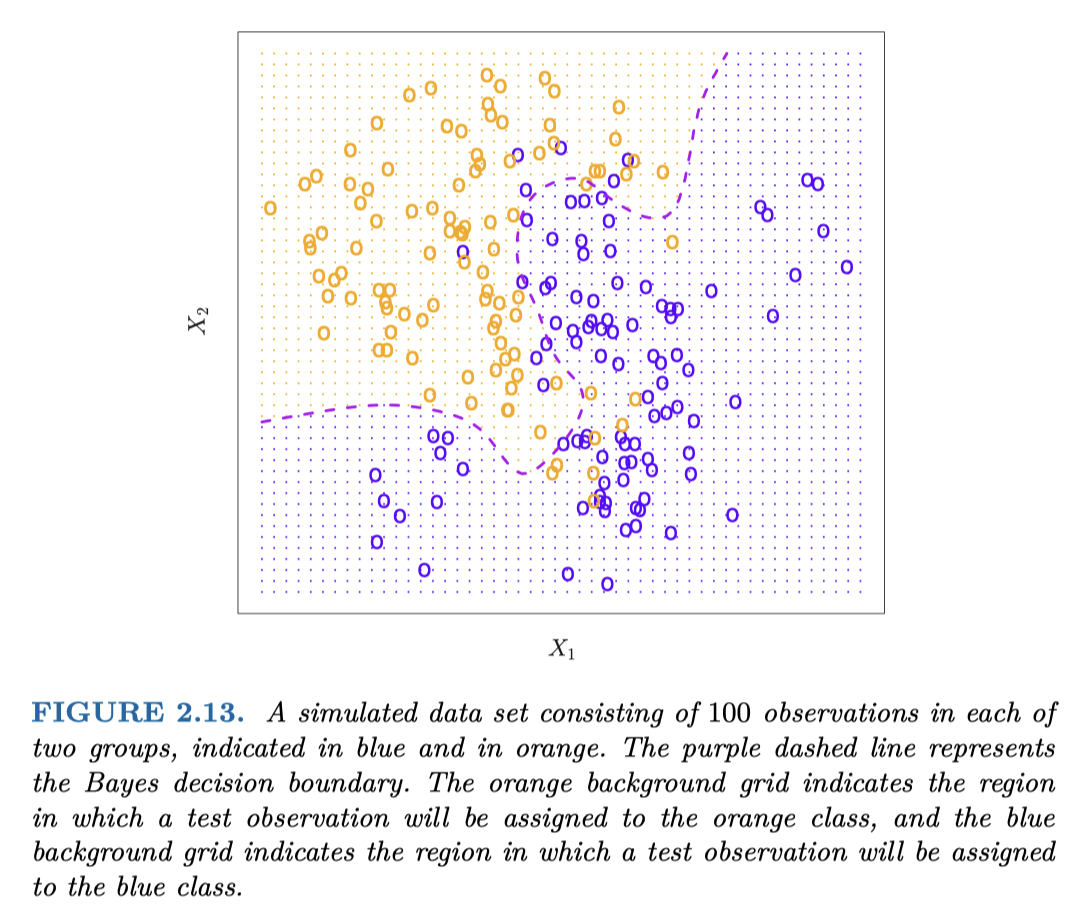
\includegraphics[width=0.60\linewidth]{KNN.png}
    \label{fig:KNN}
\end{figure}

There are some misclassified data which could be observed from the graph.

\newpage

\begin{figure}[h!]
    \centering
    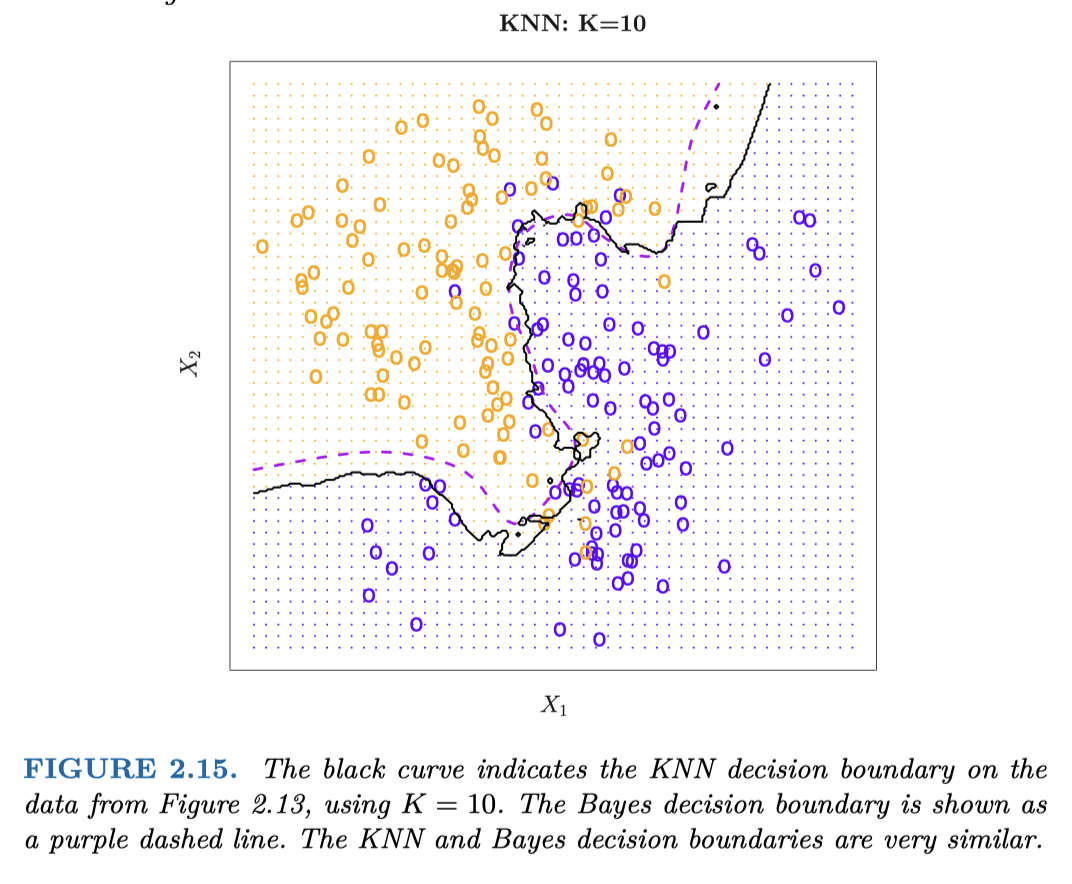
\includegraphics[width=0.5\linewidth]{KNN_10.png}
    \label{fig:KNN-10}
\end{figure}

The black curve is the estimate of the K-Nearest Neighbor with $K = 10$. The boundary is established by sampling the $10$ nearest data points of a particular data point and observe the majority color of those points.

\begin{figure}[h!]
    \centering
    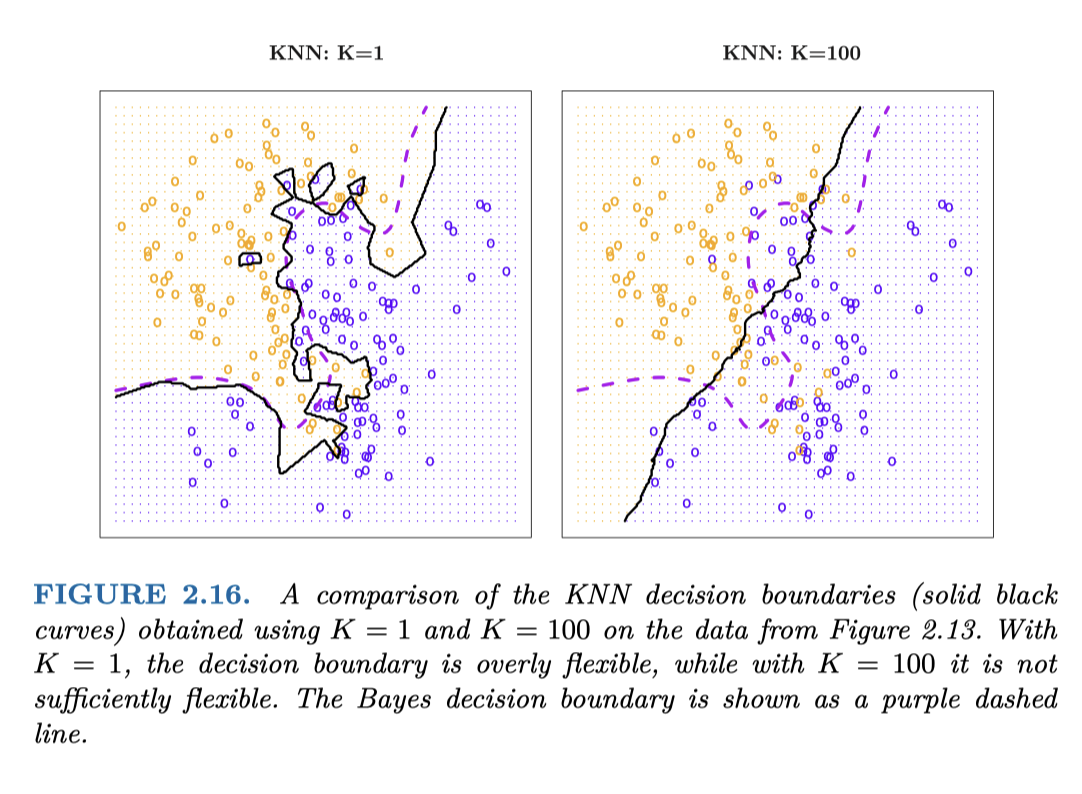
\includegraphics[width=0.75\linewidth]{KNN_compare.png}
    \label{fig:KNN-compare-1-100}
\end{figure}

The $K=1$ KNN estimate gives too much complexity which can be observed from the under-smoothed curve and islands emerged. Instead, if we use $K=100$ KNN, this model gives too little complexity which we cannot learn much from the model.
\newpage
\begin{figure}[h!]
    \centering
    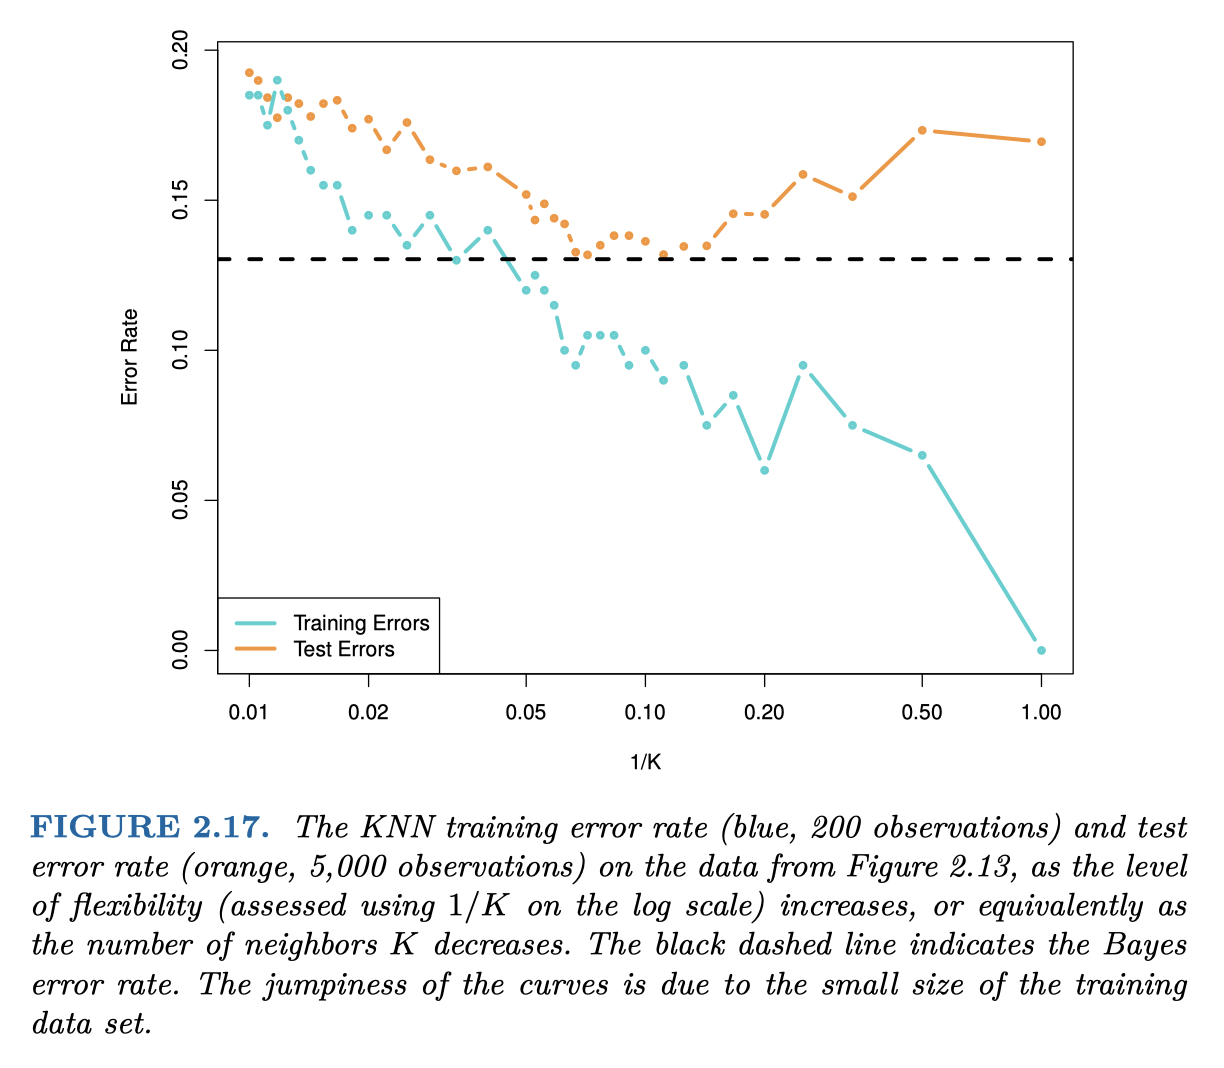
\includegraphics[width=0.75\linewidth]{Training_testing_error.png}
    \label{fig:training-testing-error}
\end{figure}

The training errors goes down as $K$ increases. However, the testing errors generally obey an U-shaped curve. We can see that $K=10$ is optimal here.

\end{document}
